\subsection{Klassediagram}
Klassediagrammet giver overblik over vores klasser i projektet. Vi har indset, at vi skal bruge mange objekter, der er variationer af samme type - f.eks. felter på spillepladen. Derfor gør vi brug af nedarvning. I tilfældet med felter er nedarvning smart, da nogle felter kan ejes af en spiller, mens andre ikke kan. Nogle felter har ingen konsekvenser (Parkeringsplads, fængsel), mens andre har (chance, start, ryk i fængsel, ejendomme).
Vi har valgt at bruge ordet \texttt{Actor} som generalisering. Dette skal ikke misforstås som aktør i kontekst af UML. I Monopoly Junior har banken egenskaber der til forveksling ligner en spillers, derfor har vi valgt at bruge nedarvning til dette, da vi bruger de samme methods til banken såvel som spilleren.
Utility er blevet flyttet udenfor diagrammet, da den ikke passer godt ind ellers. Utility bør muligvis omdøbes til Reader eller lignende, da det er mere beskrivende for hvad den gør - nemlig læser tekst- og XML-filer for at hente data til brug i andre dele af programmet. GameBoard og ChanceCardController skal begge bruge Utility for at generere adskillige objekter fra XML filer. GUIController har behov for at læse fra forskellige tekstfiler, og det bruger vi også Utility til.
\begin{figure}[h!]
\centering
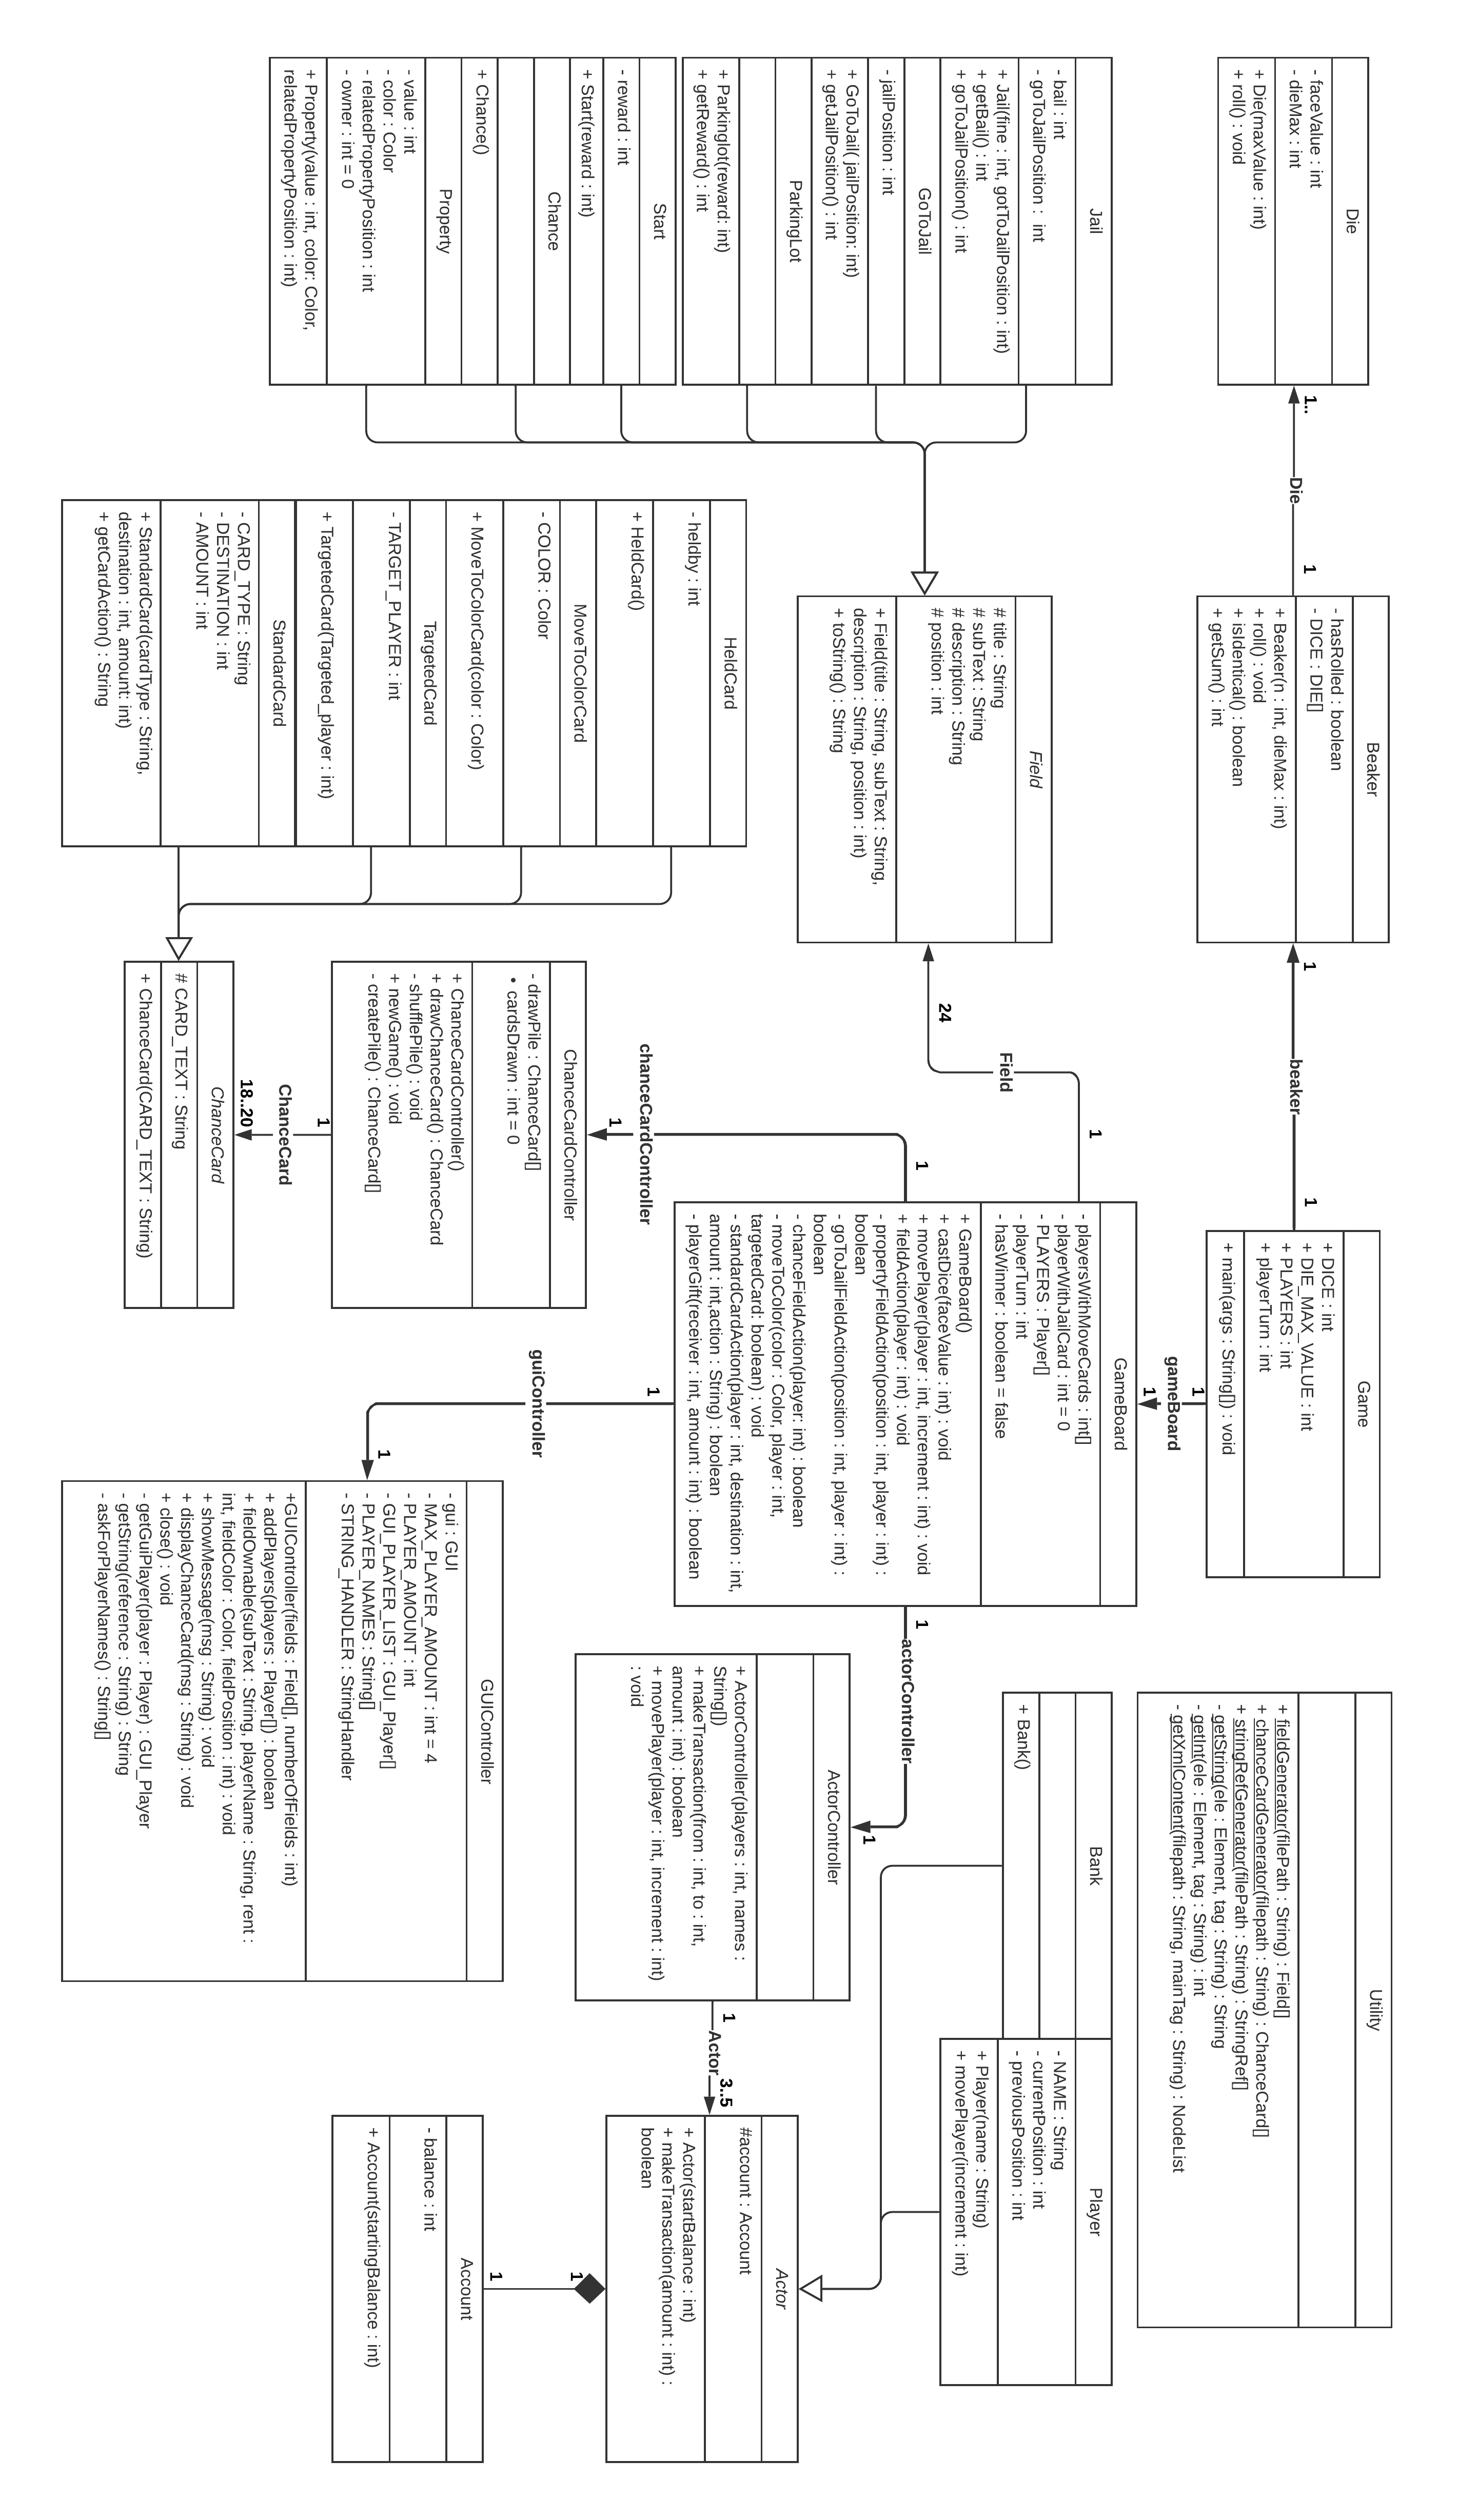
\includegraphics[scale=0.16]{artifacts/CD.png}
\end{figure}

\subsection{GUIController}
Klassen \texttt{GUIController} er den klasse som sørger for alt kommunikation til GUI’en, så vi kan nemmere hold styr på det hele ift. GRASP.
Dvs. der er kun 1 fil, man skal kigge i, når man vil kommunikere med GUI’en.
Klasse skal derud over være henholdsvis minimalistisk i den forstand af, at der skal helst ikke være mere end en 5-10 linjer kode i hver metode (nogle metoder undtaget), da det mest bare er kald, som går videre i systemet.


\subsection{ChanceCardController}
\texttt{ChanceCardController} bliver brugt til at holde styr på alle chancekort(dvs. holde en bunke kort, give mulighed for at trække et kort og blande bunken). Vi har valgt at lave en controller til dette, da det giver bedre mulighed for at overholde GRASP principperne. 
\subsection{GameBoard}
Denne klasse har vi bestemt til at være den centrale klasse der udfører det meste af handlingerne nødvendige for en spillerunde. \texttt{GameBoard} indeholder derfor både en \texttt{ActorController} til spillere og banken, en \texttt{GUIController} til at styre bruger interfacet samt et \texttt{Field} array. \texttt{GameBoard} fungerer som controller til felter, og indeholder derfor koden eksekveres for hver af felttyperne. 

Main bruger derfor kun en \texttt{Beaker} og en \texttt{GameBoard} klasse. 
\newpage
\subsection{Sekvensdiagram}
\begin{figure}[h!]
\centering
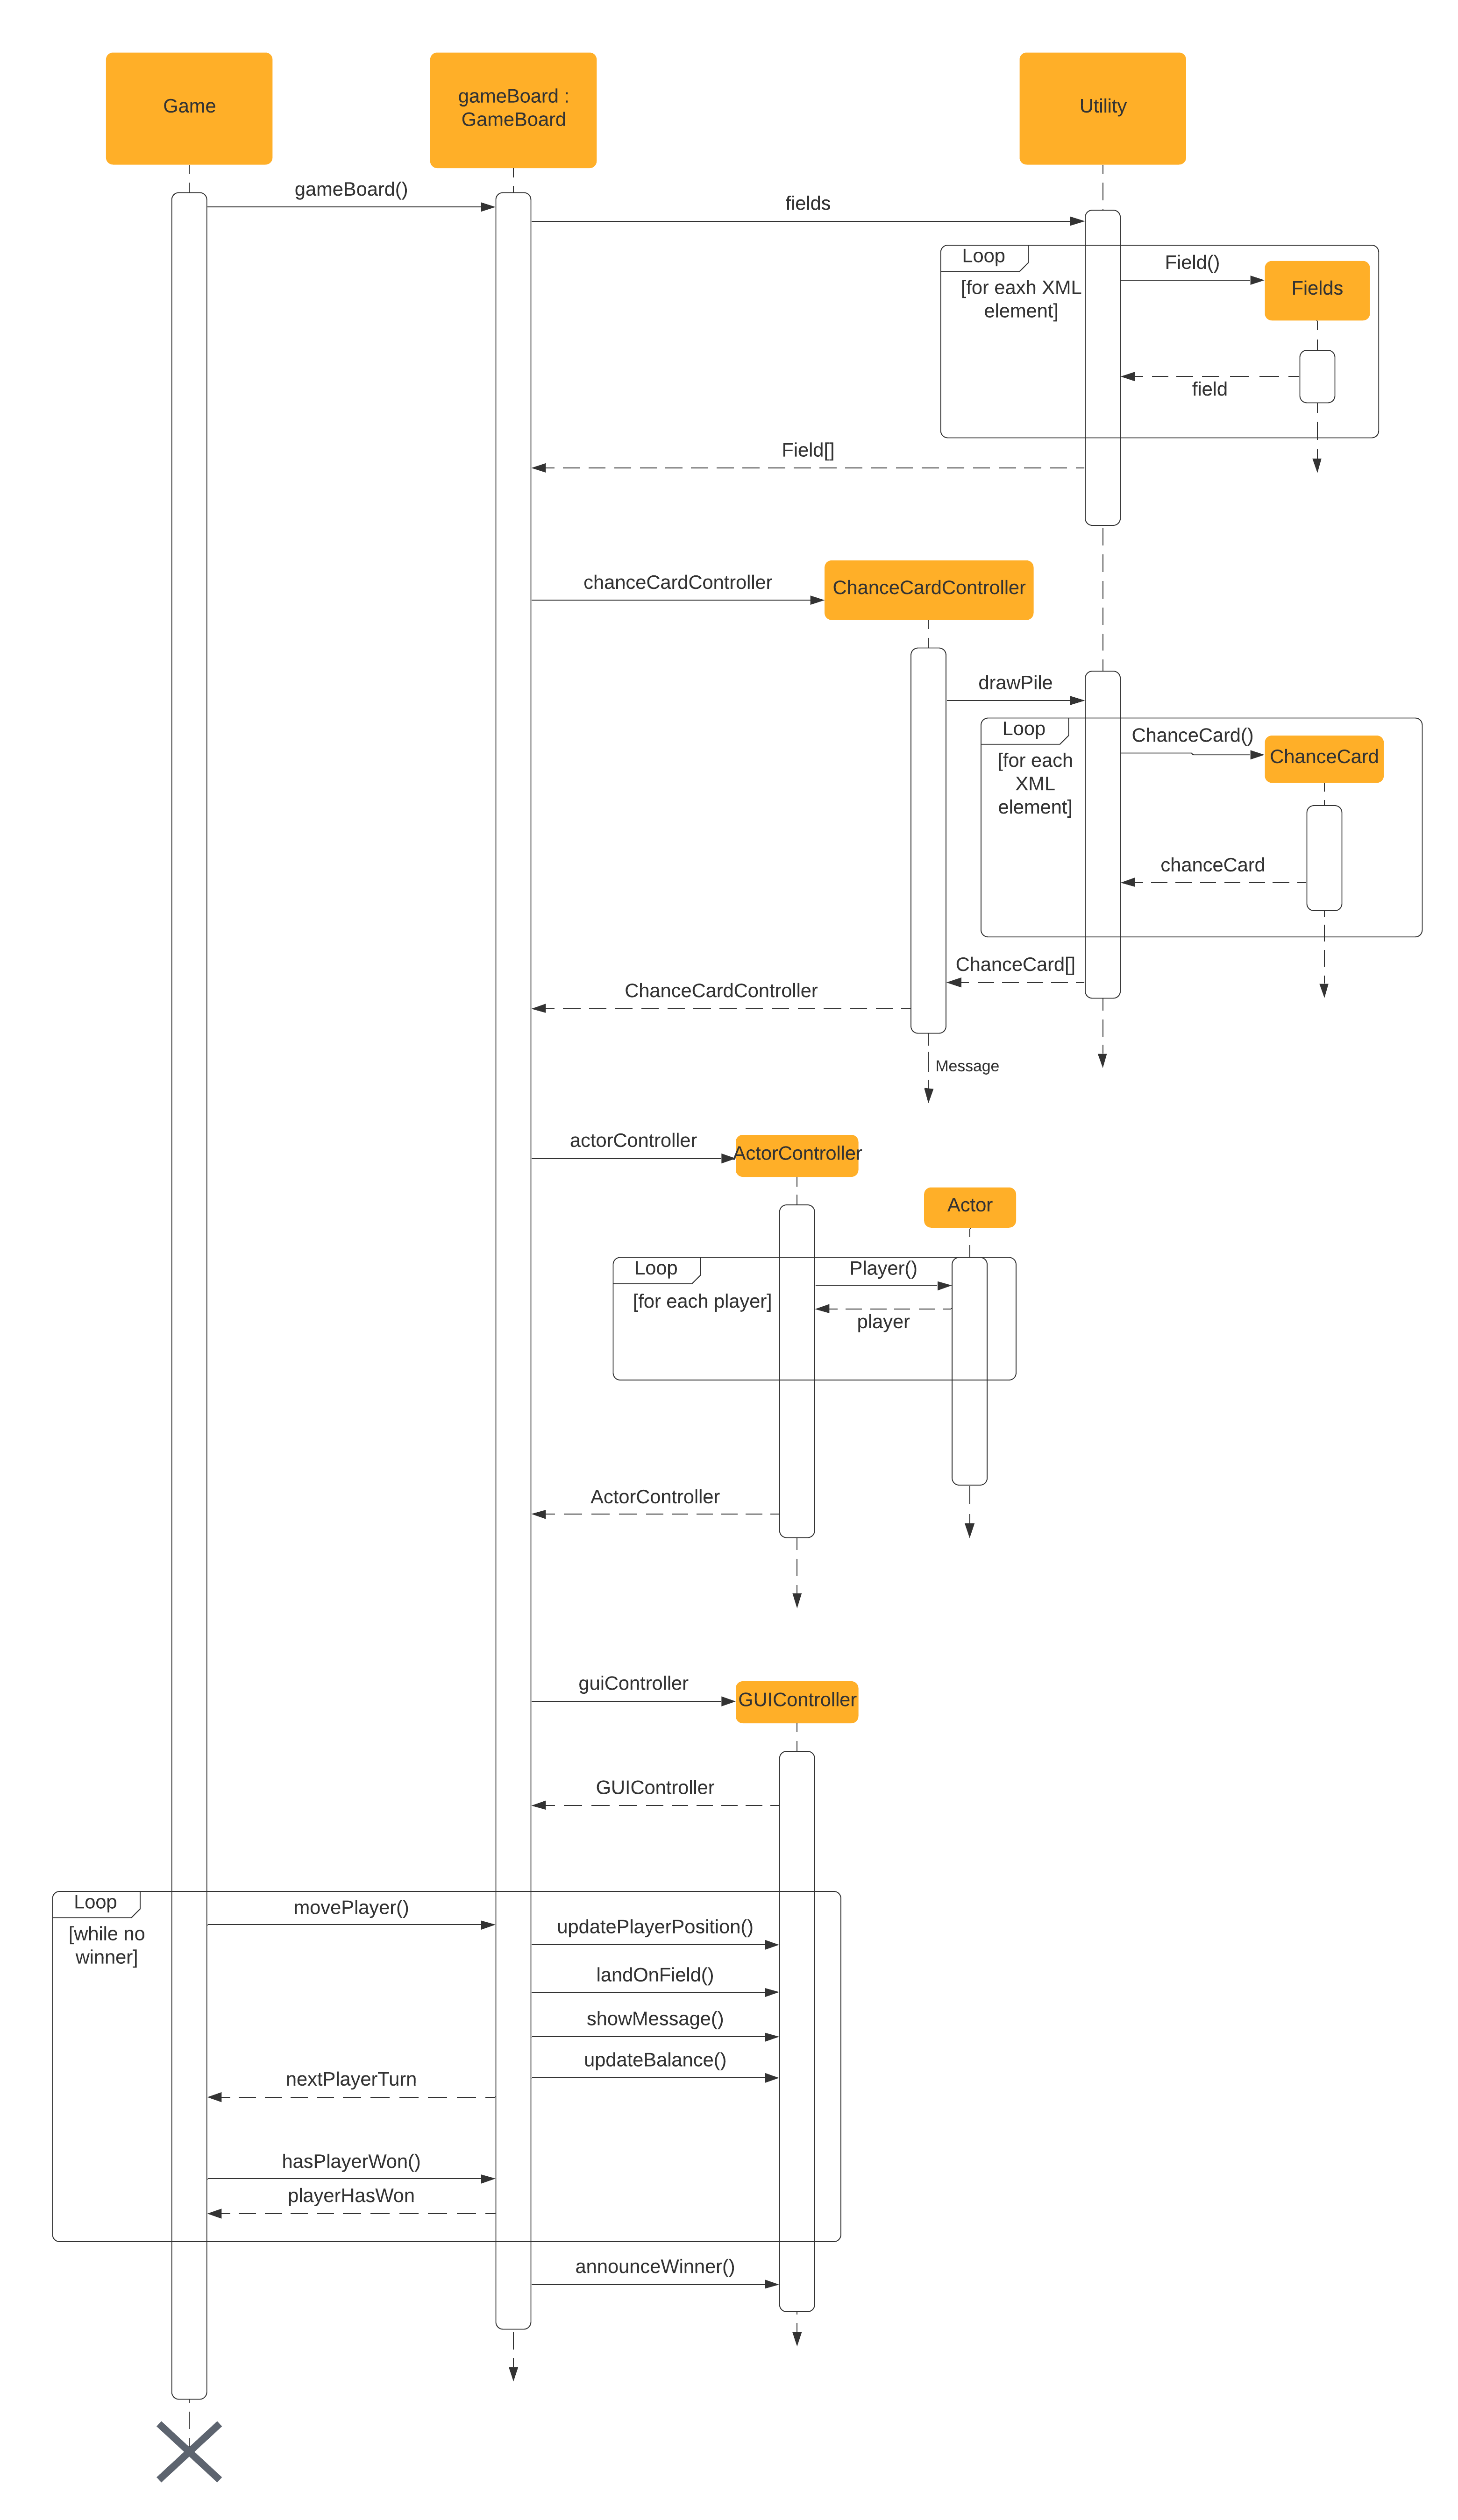
\includegraphics[scale=0.095]{artifacts/SD.png}
\end{figure}